\documentclass[11pt]{article}
\usepackage[osf,largesc,theoremfont]{newpxtext}
\usepackage[scaled=1.03]{inconsolata}
\usepackage[euler-digits,euler-hat-accent]{eulervm}
\usepackage[T1]{fontenc}
\usepackage[utf8]{inputenc}
\usepackage{graphicx}
\usepackage{float}
\usepackage{enumitem}
\usepackage{listings}
\usepackage[margin=2cm]{geometry}
\PassOptionsToPackage{hyphens}{url}
\usepackage{xcolor, colortbl}
\definecolor{BLUELINK}{HTML}{0645AD}
\definecolor{DARKBLUELINK}{HTML}{0B0080}
\definecolor{LIGHTGREY}{gray}{0.9}
\PassOptionsToPackage{hyphens}{url}
\usepackage[colorlinks=false]{hyperref}
% for linking between references, figures, TOC, etc in the pdf document
\hypersetup{colorlinks,
    linkcolor=DARKBLUELINK,
    anchorcolor=DARKBLUELINK,
    citecolor=DARKBLUELINK,
    filecolor=DARKBLUELINK,
    menucolor=DARKBLUELINK,
    urlcolor=BLUELINK
} % Color citation links in purple
\PassOptionsToPackage{unicode}{hyperref}
\PassOptionsToPackage{naturalnames}{hyperref}
\usepackage{fontawesome5}


\title{{\huge \textbf{Swiss DBC Knife}}}
\author{\textbf{Department of Computational Biology, UNIL} }
\date{\textbf{Edition 2025}}
% If you need new packages, update the file preamble.tex
% List of command for font awesome logo: https://www.ipgp.fr/~moguilny/LaTeX/fontawesome5Icons.pdf
% 

\begin{document}
% Title and logo
\maketitle
\begin{figure}[H]
    \centering
    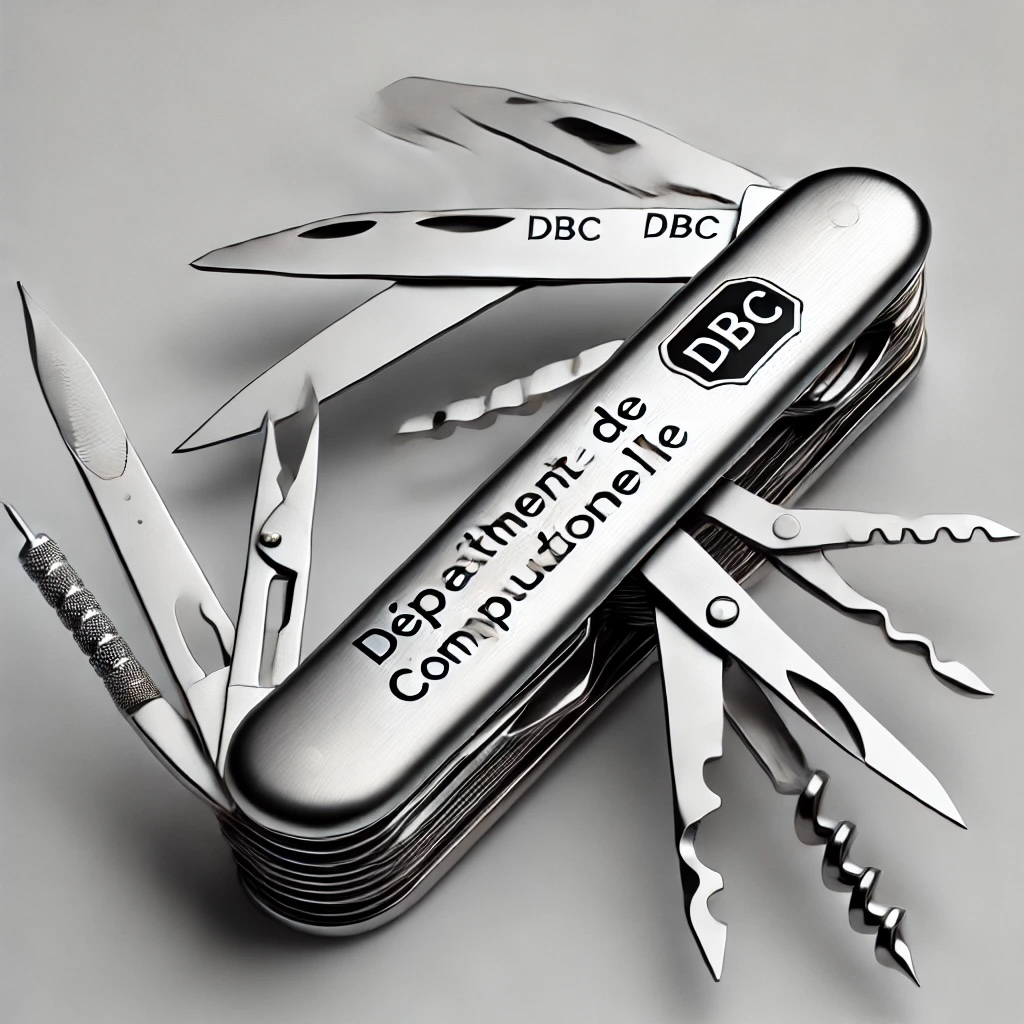
\includegraphics[width=0.3\textwidth]{images/logo.jpeg}
\end{figure}

% Summary of the goal of the document
You hold in your hands the Swiss Knife for DBC members. The goal is to have a synthetic document that contains all the information that is difficult to gather when you arrive in a new unit. This document is intended to be improved; so if you see points that could be integrated, do not hesitate to.\\

% Table of contents 
\tableofcontents
\newpage

% Make changes straight away in those files, create one if needed.
\section{Software - \faLinux/\faApple/\faWindows}
Anything related to software you can install on your computer.
\subsection{Bibliography}
There are several tools available, but Zotero stands up as open-source and community driven.
\begin{itemize}
    \item \textbf{Zotero}\ - \url{https://www.zotero.org} - \faLinux/\faApple/\faWindows.\\
    Open-source reference manager with browser extensions and integration with \LaTeX \ and Overleaf.\\
    UNIL provides unlimited storage with Zotero (see \href{https://wp.unil.ch/newsci/stockage-illimite-desormais-gratuit-sur-zotero-pour-toute-la-communaute-unil/}{this link}).
\end{itemize}

\subsection{Tree Visualisation}
Phylogenetic trees can be visualized using:
\begin{itemize}
    \item \textbf{FigTree} - \url{http://tree.bio.ed.ac.uk/software/figtree} - \faLinux/\faApple/\faWindows.\\
    Simple tree viewer for Newick files with various customization options.
\end{itemize}
\newpage
\section{Internet - \faChrome/\faFirefox/\faInternetExplorer}
Anything related to internet.

\subsection{Productivity websites}
Essential websites:
\begin{itemize}
    \item \textbf{Overleaf} - \url{https://www.overleaf.com} - \LaTeX.\\
    An online LaTeX editor that's easy to use. No installation, real-time collaboration, version control, hundreds of LaTeX templates, direct submission to biorxiv.\\
    UNIL provides a professional account (see \href{https://www.overleaf.com/edu/unil}{this link}).
\end{itemize}

\subsection{Bioinformatic websites}
Essential websites:
\begin{itemize}
    \item \textbf{Ensembl} - \url{https://www.ensembl.org}.\\
    Genome browser for vertebrate and model organism genomes.
\end{itemize}

\subsection{Browser Extensions}
Useful extensions:
\begin{itemize}
    \item \textbf{uBlock Origin} - \url{https://ublockorigin.com} - \faChrome/\faFirefox/\faInternetExplorer.\\
    Lightweight and efficient ad blocker that enhances privacy and speeds up browsing.
    \item \textbf{Zotero Connector}- \url{https://www.zotero.org/download/connectors} - \faChrome/\faFirefox/\faInternetExplorer.\\
    Enables one-click reference collection from journal articles and web pages.
\end{itemize}

\subsection{Email: Thunderbird}
Mozilla Thunderbird (\url{https://www.thunderbird.net/}) is an open-source email client that supports IMAP and SMTP. It allows integration with calendars, encryption, and robust spam filtering.

\newpage
\section{Programming and Writing Code - \faCode}
\subsection{Editor - \faEdit}
Common code editors:
\begin{itemize}
    \item \textbf{VSCode} -  \url{https://code.visualstudio.com} - \faLinux/\faApple/\faWindows/\faChrome/\faFirefox/\faInternetExplorer.\\
    Lightweight, highly extensible code editor with integrated Git support and debugging tools.
    \item \textbf{PyCharm} - \url{https://www.jetbrains.com/pycharm} - \faLinux/\faApple/\faWindows.\\
    Python IDE with built-in debugging, testing, and package management.
    \item \textbf{Sublime Text} - \url{https://www.sublimetext.com} - \faLinux/\faApple/\faWindows.\\
    Fast and responsive editor with powerful search and syntax highlighting.
\end{itemize}

\subsection{Bash and Shell - \faTerminal}
Cool shells:
\begin{itemize}
    \item \textbf{Oh My ZSH!} - \url{https://ohmyz.sh}.\\
    Open source, community-driven framework for managing your Zsh configuration. 
\end{itemize}

\subsection{Python - \faPython}
Popular libraries:
\begin{itemize}
    \item \textbf{Biopython} - \url{https://biopython.org}.\\
    Provides tools for biological computation, including sequence parsing and BLAST search.
    \item \textbf{Matplotlib} - \url{https://matplotlib.org}.\\
    Visualization library for creating static, animated, and interactive plots.
    \item \textbf{Seaborn} - \url{https://seaborn.pydata.org}.\\
    High-level statistical data visualization library.
\end{itemize}
\newpage
\section{Packaging a Software or a Piece of Code - \faBoxOpen}
\subsection{GitHub - \faGithub }
Versionned repository.

\subsection{Conda}
Create a Conda packages

\subsection{Pip - \faPython}
Create a pip package.

\subsection{Containers - \faDocker}
Create a docker container.


\newpage
\section{HPC Tricks and Tips}
It is not to replace the DSCR information, it is about our tricks and tips that we want to share. 
\subsection{DSCR Links}

\subsection{Screen}
Keep sessions running after disconnection:
\begin{lstlisting}
screen -S mysession
# To detach: Ctrl+A, then D
screen -r mysession  # Reattach session
\end{lstlisting}

\subsection{Mounting remote folder}
Mount remote directories using \texttt{sshfs}:
\begin{lstlisting}
sshfs user@remote:/path/to/dir /mnt/localmount
\end{lstlisting}

\newpage
\section{AI/ML}
\subsection{Local Models}
Run ML models locally with:
\begin{itemize}
    \item \textbf{Ollama} - \url{https://www.ollama.com} - \faLinux/\faApple/\faWindows.\\
    Get up and running with large language models. Run Llama 3.3, DeepSeek-R1, Phi-4, Mistral, Gemma 2, and other models, locally.

\end{itemize}

\subsection{Coding Assistant}
AI coding assistants:
\begin{itemize}
    \item \textbf{GitHub Copilot} - \url{https://github.com/features/copilot}.\\
    By the company OpenAI (i.e. CloseAI), integrates with VSCode and JetBrains IDE.
\end{itemize}

\newpage
\section{Courses}
\subsection{SIB}
The Swiss Institute of Bioinformatics (\url{https://www.sib.swiss/training}) offers workshops and courses on genomics, transcriptomics, and data science.

\subsection{UNIL}
UNIL (\url{https://www.unil.ch/}) provides courses.

\subsection{Online}
Available platforms:
\begin{itemize}
    \item \textbf{Coursera}, \url{https://www.coursera.org/}.\\
    Offers bioinformatics and machine learning courses from universities.
\end{itemize}

\end{document}